\documentclass[conference]{IEEEtran}
\IEEEoverridecommandlockouts

\usepackage[T1]{fontenc}
\usepackage{amsmath,amssymb}
\usepackage{graphicx}
\usepackage{booktabs}
\usepackage{xcolor}
\usepackage{tikz}
\usetikzlibrary{positioning,arrows.meta,fit,calc}
\usepackage{cite}
\usepackage[hidelinks]{hyperref}

\definecolor{lowvol}{HTML}{17745E}
\definecolor{elevated}{HTML}{A56B25}
\definecolor{stress}{HTML}{B23A3A}
\definecolor{ink}{HTML}{1B1B1B}
\definecolor{fan}{HTML}{2F4B7C}
\definecolor{boxfill}{HTML}{F3F5F8}

\newcommand{\Dmax}{D_{\max}}
\newcommand{\ind}{\mathbf{1}}
\newcommand{\Normal}{\mathcal{N}}

\begin{document}

\title{Duration-Aware Volatility Regimes for S\&P~500 Risk Scenarios: An Explicit-Duration HSMM and Its Walk-Forward Evaluation}

\author{\IEEEauthorblockN{Aditya Channa, Dr. Pooja Gupta, Madhav Kapoor, and Jastej Singh}
\IEEEauthorblockA{Department of Computer Science and Technology\\
Maharaja Agrasen Institute of Technology, New Delhi, India}}

\maketitle

\begin{abstract}
Regime-switching models of equity markets usually imply geometric state durations, so the chance of leaving a regime does not depend on how long it has lasted. We test whether an explicit-duration alternative produces better short-horizon return intervals for the S\&P~500 index. The AlphaSharp system fits a three-state Gaussian hidden semi-Markov model (HSMM) to daily log returns, log 21-session realized volatility and log VIX. Segment durations follow shifted negative binomial distributions, and the filter tracks the joint posterior of state and elapsed age. Each annual model vintage uses only the preceding ten years of data. A duration cap of 252 sessions was selected on 2000--2006 forecasts, and 2007--2025 was held out. Over 4,779 one-session forecast origins, the nominal 90\% HSMM intervals covered 89.64\% of outcomes. Mean interval scores at horizons of 1, 5 and 21 sessions were 0.05186, 0.10567 and 0.21161 for the HSMM, 0.05178, 0.10553 and 0.21086 for a matched hidden Markov model, and 0.04784, 0.09848 and 0.20088 for an exponentially weighted moving average (EWMA) volatility model. Paired block-bootstrap intervals contain zero for every HSMM--HMM difference and exclude zero for the EWMA comparison at 1 and 5 sessions. Conditioning scenarios on elapsed regime age did not improve interval scores. We report this negative result together with the application that serves the evaluated model, replays past dates, and displays the evaluation evidence beside each scenario.
\end{abstract}

\begin{IEEEkeywords}
hidden semi-Markov model, market regimes, probabilistic forecasting, interval score, walk-forward evaluation, value at risk
\end{IEEEkeywords}

%=====================================================================
\section{Introduction}
%=====================================================================
Daily equity returns are close to serially uncorrelated, but their magnitudes are not. Volatility clusters, and calm or turbulent periods persist for weeks to months~\cite{engle1982,bollerslev1986}. Regime-switching models describe this persistence with a latent discrete state whose value changes the return distribution~\cite{hamilton1989,ang2012}. In a first-order hidden Markov model (HMM), the time spent in a state is geometrically distributed. The probability of leaving a state is therefore the same on its first day and on its hundredth. Ryd\'en \emph{et al.}~\cite{ryden1998} found that this restriction limits how well HMMs reproduce the slow decay of autocorrelation in absolute returns. Bulla and Bulla~\cite{bulla2006} showed that hidden semi-Markov models (HSMMs) with flexible sojourn distributions reproduce these stylized facts more closely.

Duration dependence matters for risk scenarios. Suppose a high-volatility state has lasted 40 sessions and such states rarely last much longer. A duration-aware model then assigns a higher exit probability over the next month than it would to a state that began yesterday. An HMM cannot represent this difference. Whether it improves forecasts of index returns is an empirical question, and it is the question this paper tests.

AlphaSharp is a research application for S\&P~500 regimes and loss scenarios. Its model is a three-state explicit-duration Gaussian HSMM. Fig.~\ref{fig:arch} shows how the model is trained offline and served to a browser. This paper makes three contributions:
\begin{enumerate}
\item An HSMM whose filter retains the joint posterior over state and elapsed age, with a survival-weighted prior for the unknown initial age, a right-censored final segment, and scenario simulation conditioned on age (Section~\ref{sec:model}).
\item A walk-forward evaluation over 2007--2025 against four baselines using interval scores, coverage, Brier scores and paired block-bootstrap intervals (Sections~\ref{sec:protocol} and~\ref{sec:results}). The HSMM did not outperform a matched HMM or an EWMA volatility model.
\item An application that serves only evaluated model vintages, replays historical dates with the vintage available at the time, and shows measured baseline performance next to every scenario (Section~\ref{sec:system}).
\end{enumerate}

\begin{figure}[t]
\centering
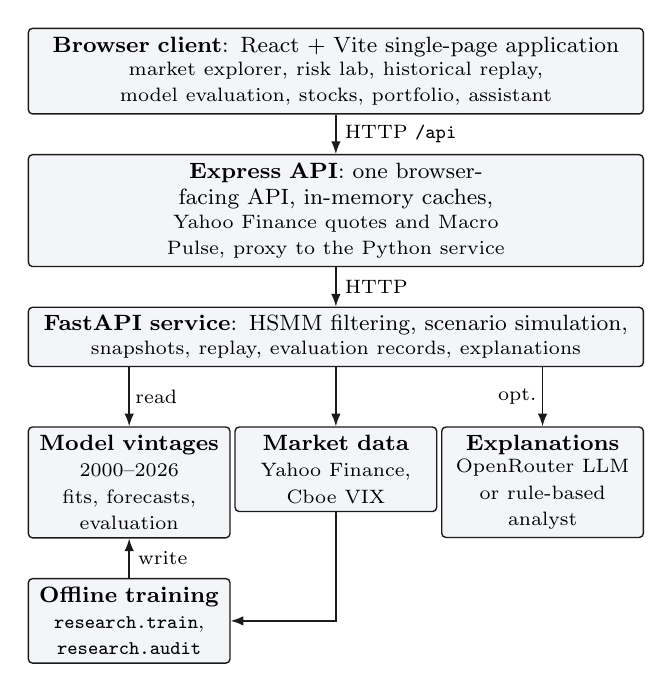
\begin{tikzpicture}[
  font=\footnotesize,
  box/.style={draw=ink, line width=0.5pt, fill=boxfill, rounded corners=1.5pt, align=center, inner sep=3pt},
  sbox/.style={box, text width=2.35cm, minimum height=0.95cm},
  arr/.style={-{Latex[length=1.6mm]}, line width=0.5pt, draw=ink},
  lab/.style={font=\scriptsize, fill=white, inner sep=1pt}
]
\node[box, text width=7.6cm] (ui) {\textbf{Browser client}: React + Vite single-page application\\[-1pt]
\scriptsize market explorer, risk lab, historical replay, model evaluation, stocks, portfolio, assistant};
\node[box, text width=7.6cm, below=0.5cm of ui] (ex) {\textbf{Express API}: one browser-facing API, in-memory caches,\\[-1pt]
\scriptsize Yahoo Finance quotes and Macro Pulse, proxy to the Python service};
\node[box, text width=7.6cm, below=0.5cm of ex] (py) {\textbf{FastAPI service}: HSMM filtering, scenario simulation,\\[-1pt]
\scriptsize snapshots, replay, evaluation records, explanations};
\node[sbox, below=0.75cm of py.south west, anchor=north west] (art) {\textbf{Model vintages}\\ \scriptsize 2000--2026 fits, forecasts, evaluation};
\node[sbox, below=0.75cm of py.south, anchor=north] (mkt) {\textbf{Market data}\\ \scriptsize Yahoo Finance, Cboe VIX};
\node[sbox, below=0.75cm of py.south east, anchor=north east] (llm) {\textbf{Explanations}\\ \scriptsize OpenRouter LLM\\ or rule-based analyst};
\node[box, text width=2.35cm, minimum height=0.95cm, below=0.5cm of art] (train) {\textbf{Offline training}\\ \scriptsize \texttt{research.train}, \texttt{research.audit}};
\draw[arr] (ui) -- node[lab, right=2pt] {HTTP \texttt{/api}} (ex);
\draw[arr] (ex) -- node[lab, right=2pt] {HTTP} (py);
\draw[arr] (py.south -| art.north) -- node[lab, right=1pt] {read} (art.north);
\draw[arr] (py.south) -- (mkt.north);
\draw[arr] (py.south -| llm.north) -- node[lab, left=1pt] {opt.} (llm.north);
\draw[arr] (train) -- node[lab, right=2pt] {write} (art);
\draw[arr] (mkt.south) |- (train.east);
\end{tikzpicture}
\caption{AlphaSharp architecture. Training and evaluation run offline and write versioned model vintages. The online services only read those artifacts; the language model is optional and is replaced by a rule-based analyst when no key is configured.}
\label{fig:arch}
\end{figure}

%=====================================================================
\section{Related Work}
%=====================================================================
\textit{Regime models.} Hamilton~\cite{hamilton1989} introduced Markov-switching autoregressions for nonstationary economic series, and Rabiner~\cite{rabiner1989} gave the standard treatment of HMM inference and estimation. Parameters are usually estimated with the expectation-maximization (EM) algorithm~\cite{dempster1977}. Ang and Timmermann~\cite{ang2012} survey regime models in finance and note that regimes are frequently identified by volatility rather than by mean return. Ryd\'en \emph{et al.}~\cite{ryden1998} fitted HMMs to daily returns and reported that they fail to reproduce the long memory of absolute returns.

\textit{Hidden semi-Markov models.} An HSMM assigns each state an explicit sojourn distribution. Yu~\cite{yu2010} surveys HSMM formulations and inference algorithms, including the expanded state-and-age representation that we use. Gu\'edon~\cite{guedon2003} derived EM estimation for hidden semi-Markov chains with right-censored final sojourns. Bulla and Bulla~\cite{bulla2006} applied HSMMs with negative binomial and other sojourn laws to daily index returns and found that they reproduce stylized facts better than HMMs. Our model follows this line but uses multivariate emissions that include implied volatility and evaluates out-of-sample interval forecasts rather than in-sample fit.

\textit{Volatility forecasting.} ARCH and GARCH models~\cite{engle1982,bollerslev1986} make conditional variance a function of past squared returns. The RiskMetrics method~\cite{riskmetrics1996} uses an exponentially weighted moving average of squared returns with decay $\lambda=0.94$ for daily data and is a standard benchmark for short-horizon risk. We use it as a baseline because it adapts to every new return, whereas a three-state model can only move between three variance levels.

\textit{Forecast evaluation and risk measures.} Gneiting and Raftery~\cite{gneiting2007} define the interval score as a proper scoring rule for central prediction intervals. It rewards narrow intervals and penalizes misses in proportion to their size. Christoffersen~\cite{christoffersen1998} formalized coverage tests for interval forecasts, and Brier~\cite{brier1950} introduced the quadratic score for probability forecasts. Diebold and Mariano~\cite{diebold1995} framed comparisons of predictive accuracy as tests on loss differentials. Because daily loss differentials are serially dependent, we form confidence intervals with the moving-block bootstrap of K\"unsch~\cite{kunsch1989}; the stationary bootstrap of Politis and Romano~\cite{politis1994} is a common alternative. Artzner \emph{et al.}~\cite{artzner1999} gave axioms for coherent risk measures and showed that value at risk (VaR) can violate subadditivity. The application therefore reports expected shortfall beside VaR.

%=====================================================================
\section{Data}
\label{sec:data}
%=====================================================================
Daily closes of the S\&P~500 price index come from Yahoo Finance, and VIX closes come from Cboe's published history~\cite{cboevix}. The snapshot used here covers 2 January 1990 to 30 October 2026, with 9,272 sessions on which both series are available. Yahoo and Cboe VIX closes agree to within 0.05 points on 99.90\% of these sessions. Nine sessions differ by more than 0.05, with a maximum absolute difference of 2.61 points; the Cboe value is used throughout. S\&P~500 closes were compared with the FRED series SP500~\cite{fred}. Of 2,512 overlapping sessions, 99.88\% agree to within 0.1 index points, and the largest difference is 5.29 points. Missing observations are dropped, not forward-filled. The index excludes dividends.

Evaluation uses a frozen file of 9,063 sessions from 2 January 1990 to 31 December 2025. Its SHA-256 hash is stored with the results so that later price refreshes cannot change the evaluation. Let $P_t$ be the index close on session $t$. The model observes the vector $\mathbf{y}_t=(r_t, v_t, z_t)^\top$ with
\begin{equation}
r_t=\ln\frac{P_t}{P_{t-1}},\quad
v_t=\ln\!\big(\sqrt{252}\,\hat\sigma_t\big),\quad
z_t=\ln \mathrm{VIX}_t,
\label{eq:features}
\end{equation}
where $\hat\sigma_t$ is the sample standard deviation of $r_{t-20},\dots,r_t$. The first complete feature vector is on 31 January 1990. Each vintage standardizes $\mathbf{x}_t=\mathrm{diag}(\mathbf{s})^{-1}(\mathbf{y}_t-\mathbf{m})$, where $\mathbf{m}$ and $\mathbf{s}$ are the mean and standard deviation over that vintage's training window only. Forecast targets are simple returns $R_{t,h}=P_{t+h}/P_t-1$ over $h$ sessions.

%=====================================================================
\section{Model}
\label{sec:model}
%=====================================================================
\subsection{Explicit-duration HSMM}
The hidden process at session $t$ is the pair $(S_t, A_t)$. The state $S_t\in\{1,2,3\}$ indexes a volatility regime, and the age $A_t\in\{0,\dots,\Dmax-1\}$ counts the sessions already completed in the current segment. Given the state, observations are Gaussian:
\begin{equation}
\mathbf{x}_t \mid S_t=k \;\sim\; \Normal(\boldsymbol\mu_k, \boldsymbol\Sigma_k).
\label{eq:emission}
\end{equation}
We write $b_k(\mathbf{x}_t)$ for this density. A segment of state $k$ lasts $D_k$ sessions, where $D_k-1$ follows a negative binomial law with mean $m_k$ and dispersion $\rho_k$, truncated to $\{1,\dots,\Dmax\}$:
\begin{equation}
p_k(d)=\frac{1}{Z_k}\,\frac{\Gamma(d-1+\rho_k)}{\Gamma(\rho_k)\,(d-1)!}\,q_k^{\rho_k}(1-q_k)^{d-1},
\label{eq:duration}
\end{equation}
where $q_k=\rho_k/(\rho_k+m_k)$ and $Z_k$ normalizes the truncated support. The shifted form guarantees $D_k\geq 1$; the untruncated mean is $1+m_k$. A geometric duration, which an HMM implies, is the special case $\rho_k=1$. Exits are governed by the hazard
\begin{equation}
h_k(a)=\frac{p_k(a+1)}{\sum_{d\geq a+1}p_k(d)},\qquad h_k(\Dmax-1)=1,
\label{eq:hazard}
\end{equation}
the probability that a segment of age $a$ ends after the current session. When a segment ends, the next state is drawn from a transition matrix $\mathbf{T}$ with $T_{kk}=0$. Self-persistence is therefore carried entirely by \eqref{eq:duration}.

\subsection{Filtering over state and age}
Let $\alpha_t(k,a)=\Pr(S_t=k, A_t=a\mid \mathbf{x}_{1:t})$. The forward recursion is
\begin{align}
\alpha_t(k,0) &= \frac{b_k(\mathbf{x}_t)}{c_t}\sum_{j} T_{jk}\sum_{a'} h_j(a')\,\alpha_{t-1}(j,a'), \label{eq:fwd0}\\
\alpha_t(k,a) &= \frac{b_k(\mathbf{x}_t)}{c_t}\,\big(1-h_k(a-1)\big)\,\alpha_{t-1}(k,a-1), \label{eq:fwda}
\end{align}
with \eqref{eq:fwda} applying for $a\geq 1$. Here $c_t$ makes $\alpha_t$ sum to one and $\sum_t \ln c_t$, plus the per-session constants removed when emissions are rescaled for numerical stability, is the log-likelihood. The filtered state probability is $\sum_a \alpha_t(k,a)$. The application also reports the expected age $\sum_a (a+1)\,\alpha_t(k,a)/\sum_a \alpha_t(k,a)$ and the probability $\sum_{k,a} h_k(a)\,\alpha_t(k,a)$ that the current segment ends after this session. Each step costs $O(K^2+K\Dmax)$ operations for $K=3$ states.

The age at the start of a training window is unknown, because the window usually begins inside a segment. Rather than assume a fresh segment, the filter starts from the survival-weighted prior
\begin{equation}
\pi(k,a)=\frac{\Pr(D_k^{(0)}\geq a+1)}{\sum_{j}\mathbb{E}\big[D_j^{(0)}\big]},
\label{eq:prior}
\end{equation}
so that $\alpha_1(k,a)\propto \pi(k,a)\,b_k(\mathbf{x}_1)$. Within a state, \eqref{eq:prior} is the equilibrium age distribution of a renewal process with duration law $p_k$. Across states it weights each state by its expected duration. The superscript $(0)$ indicates that $\pi$ is computed once from the initial duration parameters and held fixed during estimation.

\subsection{Estimation}
Parameters are estimated by EM~\cite{dempster1977,guedon2003}. The backward pass starts from $\beta_T(k,a)=1$ for every state and age. The final segment is therefore right-censored: the likelihood does not require it to end at the last observation. The E-step yields posterior state weights and, for each state and age, expected exit counts $E_k(a)$ and stay counts $R_k(a)$. The M-step updates $\boldsymbol\mu_k$ and $\boldsymbol\Sigma_k$ as weighted moments, adding $10^{-4}\mathbf{I}$ to each covariance. Duration parameters maximize the expected hazard log-likelihood
\begin{equation}
\mathcal{L}_k=\sum_{a}\bigl[E_k(a)\ln h_k(a)+R_k(a)\ln(1-h_k(a))\bigr]
\label{eq:mstep}
\end{equation}
by L-BFGS-B on $(\ln m_k,\ln\rho_k)$ with $m_k\in[0.05, 2\Dmax]$ and $\rho_k\in[0.1,100]$. $\mathbf{T}$ is set from expected transition counts with a zero diagonal. EM stops when the log-likelihood gains less than 0.01 in an iteration. An update that lowers the log-likelihood by more than $10^{-5}$ is rejected and ends the fit.

Initial values come from $k$-means clustering followed by a full-covariance Gaussian HMM. The HMM self-transition probabilities give initial mean durations, capped at $\Dmax/2$, with $\rho_k=2$. Each vintage is fitted from three seeds (7, 21 and 42), and the fit with the highest log-likelihood is kept. States are then ordered by the mean of standardized log realized volatility and labeled Low volatility, Elevated volatility and Stress.

\subsection{Scenario simulation}
Return scenarios use the marginal of the return coordinate in each state, mapped back to daily log-return units:
\begin{equation}
\mu^{r}_k=m_1+s_1\mu_{k,1},\qquad \sigma^{r}_k=s_1\sqrt{\Sigma_{k,11}}.
\label{eq:returns}
\end{equation}
For each of $N=2{,}000$ paths, $(S,A)$ is drawn from $\alpha_t$. For $\tau=1,\dots,H$, the segment ends with probability $h_S(A)$. On exit, a new state is drawn from row $S$ of $\mathbf{T}$ and $A$ is set to 0; otherwise $A\leftarrow\min(A+1,\Dmax-1)$. A daily log return $\varepsilon_\tau\sim\Normal(\mu^{r}_S,(\sigma^{r}_S)^2)$ is then drawn, and
\begin{equation}
R^{(n)}_{t,H}=\exp\Big(\sum_{\tau=1}^{H}\varepsilon_\tau\Big)-1 .
\label{eq:sim}
\end{equation}
The random seed is the origin date written as an integer, so every forecast is reproducible. Forecast quantiles and the loss probability $\hat p_t=\Pr(R_{t,H}<0)$ are read from the simulated paths. The application reports 95\% VaR as the 95th percentile of $-R_{t,H}$ and expected shortfall as the mean of $-R_{t,H}$ beyond it. Because \eqref{eq:returns} uses the marginal, simulated returns do not depend on the realized-volatility and VIX coordinates once the state is fixed.

%=====================================================================
\section{Evaluation Protocol}
\label{sec:protocol}
%=====================================================================
\subsection{Rolling vintages and configuration}
Fig.~\ref{fig:timeline} shows the design. The vintage for year $Y$ is trained on calendar years $Y-10$ to $Y-1$ and issues forecasts after each close in year $Y$. Training windows contain 2,503 to 2,523 sessions. A forecast is scored only if its outcome date falls in 2025 or earlier.

The only tuned setting is the duration cap $\Dmax\in\{126,252\}$. It was chosen on development vintages for 2000--2006, using only forecasts whose 21-session outcome window ended in 2006 or earlier. The pooled mean HSMM interval score was 0.11445 for $\Dmax=126$ and 0.11354 for $\Dmax=252$, so $\Dmax=252$ was selected. The 2007--2025 period was not used for this choice. The number of states, the ten-year window and the feature set were fixed by design and not tuned.

\begin{figure}[t]
\centering
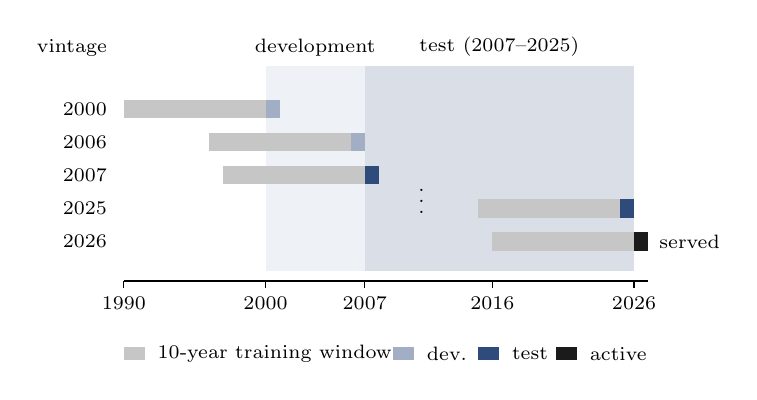
\begin{tikzpicture}[x=0.18cm, y=0.42cm, font=\scriptsize]
  % background periods
  \fill[fan!8] (10,0.3) rectangle (17,-5.9);
  \fill[fan!18] (17,0.3) rectangle (36,-5.9);
  \node[anchor=south] at (13.5,0.3) {development};
  \node[anchor=south] at (26.5,0.3) {test (2007--2025)};
  % rows: label, train start, forecast year, style
  \foreach \row/\lab/\ts/\fy/\col in {1/2000/0/10/fan!45, 2/2006/6/16/fan!45, 3/2007/7/17/fan, 4/2025/25/35/fan, 5/2026/26/36/ink}{
    \node[anchor=east] at (-0.5,-\row) {\lab};
    \fill[gray!45] (\ts,-\row+0.28) rectangle (\ts+10,-\row-0.28);
    \fill[\col] (\fy,-\row+0.28) rectangle (\fy+1,-\row-0.28);
  }
  \node at (21,-3.55) {$\vdots$};
  \node[anchor=west] at (37.1,-5) {served};
  % axis
  \draw[line width=0.4pt] (0,-6.2) -- (37,-6.2);
  \foreach \y/\lab in {0/1990,10/2000,17/2007,26/2016,36/2026}{
    \draw (\y,-6.2) -- (\y,-6.4) node[below] {\lab};
  }
  \node[anchor=south east] at (-0.5,0.3) {vintage};
  % legend
  \begin{scope}[shift={(0,-8.4)}]
    \fill[gray!45] (0,0.2) rectangle (1.5,-0.2); \node[anchor=west] at (1.7,0) {10-year training window};
    \fill[fan!45] (19,0.2) rectangle (20.5,-0.2); \node[anchor=west] at (20.7,0) {dev.};
    \fill[fan] (25,0.2) rectangle (26.5,-0.2); \node[anchor=west] at (26.7,0) {test};
    \fill[ink] (30.5,0.2) rectangle (32,-0.2); \node[anchor=west] at (32.2,0) {active};
  \end{scope}
\end{tikzpicture}
\caption{Rolling-window design. Each annual vintage is trained on the preceding ten calendar years and forecasts one year. Vintages 2000--2006 selected $\Dmax$; vintages 2007--2025 form the test. The 2026 vintage, trained on 2016--2025, is served by the application.}
\label{fig:timeline}
\end{figure}

\subsection{Baselines}
All methods forecast the same targets from the same origins. \emph{HSMM age reset} uses the fitted HSMM and its filtered state probabilities but sets every simulated age to zero, which removes the information in elapsed age. \emph{HMM} is a three-state full-covariance Gaussian HMM fitted to the same standardized features and training window, initialized in the same way and selected from the same three seeds by training log-likelihood. Its scenarios use the same return mapping \eqref{eq:returns} with Markov state transitions. \emph{Gaussian} draws independent normal log returns with the training-window mean and standard deviation. \emph{EWMA} uses the RiskMetrics recursion $\sigma_t^2=0.94\,\sigma_{t-1}^2+0.06\,r_t^2$~\cite{riskmetrics1996} with zero mean, so $\ln(1+R_{t,h})\sim\Normal(0,h\sigma_t^2)$. Its loss probability is always 0.5.

\subsection{Scores}
For the central 90\% interval $[l_t,u_t]$ formed by the 5th and 95th percentiles, the interval score~\cite{gneiting2007} with $\alpha=0.1$ is
\begin{multline}
\mathrm{IS}_t=(u_t-l_t)+\frac{2}{\alpha}(l_t-y_t)\,\ind\{y_t<l_t\}\\
+\frac{2}{\alpha}(y_t-u_t)\,\ind\{y_t>u_t\},
\label{eq:is}
\end{multline}
where $y_t=R_{t,h}$. Lower is better, and all scores are in decimal-return units. We also report coverage, mean width, the lower breach rate $\Pr(y_t<l_t)$ with nominal value 5\%, and the Brier score $(\hat p_t-\ind\{y_t<0\})^2$~\cite{brier1950} for the loss probability.

\subsection{Paired comparisons}
For each horizon and baseline $B$, let $\delta_t=\mathrm{IS}^{\mathrm{HSMM}}_t-\mathrm{IS}^{B}_t$ on common origins. Overlapping horizons and volatility clustering make $\delta_t$ serially dependent. We therefore form a 95\% percentile interval for the mean $\bar\delta$ with a moving-block bootstrap~\cite{kunsch1989} using blocks of 63 sessions and 500 resamples. We also recompute the summary scores on non-overlapping origins, taking every $h$-th origin.

\subsection{Audit}
An automated audit checks all 27 vintages from 2000 to 2026. It verifies that each training window ends before its forecast year and spans ten years, that standardization constants equal training-window moments, that the EM log-likelihood never decreases, that the stopping tolerance was reached, that all covariances are positive definite, and that every saved outcome equals the ratio of future and current closes. The audit initially found that the 2013 fit had stopped at the original 30-iteration limit while still improving. The limit was raised to 200 and only that vintage was refitted; it converged after 49 iterations, and its forecasts were regenerated. This correction was made after the evaluation results had been inspected, so the 2013 test year is not an untouched holdout. All 27 vintages pass the audit. The test vintages converged in 5 to 49 iterations.

%=====================================================================
\section{Results}
\label{sec:results}
%=====================================================================
\subsection{Estimated regimes}
Table~\ref{tab:states} summarizes the active 2026 vintage, trained on 4 January 2016 to 31 December 2025 (2,514 sessions). The three seeds reached the same log-likelihood, $-6625.644$, to within $10^{-6}$. Daily return standard deviation rises from 0.512\% in Low volatility to 0.923\% in Elevated volatility and 1.947\% in Stress. Only Stress has a negative mean daily return. Fig.~\ref{fig:dur} shows the fitted duration laws. Low-volatility segments have a mean of 55.6 sessions and a 33.5\% probability of exceeding 63 sessions. Elevated segments are shorter and more regular ($\rho=3.05$). Stress has $\rho=0.48<1$, which gives a mode at one session ($p(1)=0.17$), a median of 9 sessions and a heavier tail than Elevated. A dispersion below one means that the hazard of leaving Stress falls as a segment ages, over most of the support below the cap. A geometric law cannot express this.

\begin{table}[t]
\centering
\caption{Active 2026 vintage: state parameters}
\label{tab:states}
\footnotesize
\setlength{\tabcolsep}{4pt}
\begin{tabular}{@{}lrrr@{}}
\toprule
 & Low vol. & Elevated & Stress \\
\midrule
Mean daily log return $\mu^r_k$ (\%) & 0.091 & 0.093 & $-0.089$ \\
Daily std.\ dev.\ $\sigma^r_k$ (\%) & 0.512 & 0.923 & 1.947 \\
Realized volatility, ann.\ (\%)$^\dagger$ & 8.49 & 16.08 & 20.64 \\
VIX level$^\dagger$ & 13.18 & 18.29 & 27.00 \\
Duration mean $\mathbb{E}[D_k]$ (sessions) & 55.6 & 22.3 & 18.7 \\
Duration median (sessions) & 45 & 20 & 9 \\
Dispersion $\rho_k$ & 1.51 & 3.05 & 0.48 \\
$\Pr(D_k>63)$ & 0.335 & 0.009 & 0.063 \\
\bottomrule
\end{tabular}

\vspace{2pt}
\parbox{\columnwidth}{\scriptsize $^\dagger$Exponential of the state mean of the log feature, i.e., a geometric-mean level. Durations are for the truncated law with $\Dmax=252$.}
\end{table}

\begin{figure}[t]
\centering
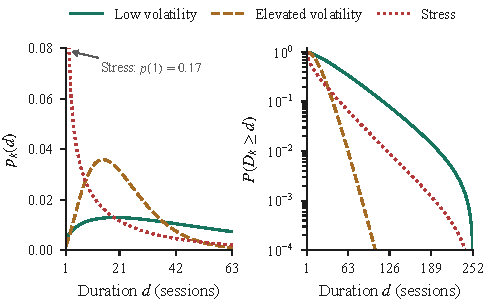
\includegraphics[width=\columnwidth]{figures/fig_durations.pdf}
\caption{Fitted duration distributions of the active 2026 vintage. Left: probability mass $p_k(d)$ for $d\le 63$; the Stress mass at $d=1$ is off the axis. Right: survival $\Pr(D_k\ge d)$ on a log scale up to the cap $\Dmax=252$.}
\label{fig:dur}
\end{figure}

The off-diagonal transition probabilities of this vintage are 0.305 (Low to Elevated), 0.695 (Low to Stress), 0.485 (Elevated to Low), 0.515 (Elevated to Stress), 0.093 (Stress to Low) and 0.907 (Stress to Elevated). Most Low segments therefore end in Stress, and the geometric-mean realized volatility in Stress is 20.64\%. Together with the short median duration, this indicates that the Stress state captures brief volatility bursts from calm markets as well as prolonged crises.

Fig.~\ref{fig:regimes} stitches the filtered labels of the 19 test vintages, each applied only to its own forecast year. Of 4,780 sessions in 2007--2025, the most probable state was Low volatility on 40.7\%, Elevated on 35.5\% and Stress on 23.8\%, and the label changed 167 times. As sanity checks against observed VIX, the model assigns Stress with probability above 0.999 on 20 November 2008 (VIX 80.86), 16 March 2020 (VIX 82.69) and 7 March 2022 (VIX 36.45), and Low volatility with probability above 0.9999 on 3 July 2017 (VIX 11.22). These are consistency checks, not accuracy measurements, because there are no ground-truth regime labels.

\begin{figure*}[t]
\centering
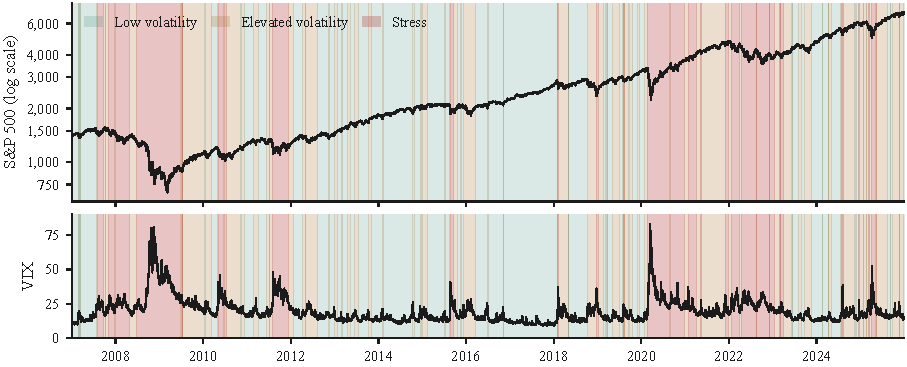
\includegraphics[width=\textwidth]{figures/fig_regimes.pdf}
\caption{S\&P~500 close (top, log scale) and VIX (bottom) over the test period, shaded by the most probable filtered state. Each year's labels come from the vintage trained on the preceding ten years and use only observations available on that day.}
\label{fig:regimes}
\end{figure*}

\subsection{Forecast accuracy}
Table~\ref{tab:overall} and Fig.~\ref{fig:scores} report the 2007--2025 results. HSMM intervals covered 89.64\%, 91.75\% and 92.75\% of outcomes at 1, 5 and 21 sessions. Coverage is close to nominal, but the misses are asymmetric. Lower breaches occurred on 6.44\%, 5.88\% and 6.16\% of origins, above the nominal 5\%, while upper breaches occurred on 3.91\%, 2.37\% and 1.09\%. The intervals are too narrow on the loss side and too wide on the gain side.

\begin{table}[t]
\centering
\caption{Test results, 2007--2025, nominal 90\% intervals}
\label{tab:overall}
\footnotesize
\setlength{\tabcolsep}{3.2pt}
\begin{tabular}{@{}llrrrrr@{}}
\toprule
$h$ & Method & Cov.\,(\%) & Breach\,(\%) & Width & IS & Brier \\
\midrule
1 & HSMM & 89.64 & 6.44 & 0.0347 & 0.05186 & 0.2491 \\
  & HSMM age reset & 89.58 & 6.51 & 0.0346 & 0.05175 & 0.2490 \\
  & HMM & 89.39 & 6.51 & 0.0346 & 0.05178 & 0.2489 \\
  & EWMA & 89.41 & 5.90 & 0.0347 & \textbf{0.04784} & 0.2500 \\
  & Gaussian & 91.46 & 4.92 & 0.0400 & 0.06095 & 0.2494 \\
\midrule
5 & HSMM & 91.75 & 5.88 & 0.0782 & 0.10567 & 0.2461 \\
  & HSMM age reset & 91.50 & 6.01 & 0.0776 & 0.10575 & 0.2460 \\
  & HMM & 91.73 & 5.93 & 0.0777 & 0.10553 & 0.2456 \\
  & EWMA & 91.04 & 5.51 & 0.0777 & \textbf{0.09848} & 0.2500 \\
  & Gaussian & 92.86 & 4.23 & 0.0895 & 0.12064 & 0.2469 \\
\midrule
21 & HSMM & 92.75 & 6.16 & 0.1638 & 0.21161 & 0.2407 \\
  & HSMM age reset & 92.10 & 6.66 & 0.1613 & 0.21170 & 0.2394 \\
  & HMM & 92.75 & 6.07 & 0.1626 & 0.21086 & 0.2385 \\
  & EWMA & 91.87 & 5.46 & 0.1597 & \textbf{0.20088} & 0.2500 \\
  & Gaussian & 94.12 & 4.16 & 0.1842 & 0.23692 & 0.2407 \\
\bottomrule
\end{tabular}

\vspace{2pt}
\parbox{\columnwidth}{\scriptsize Origins: 4,779 ($h=1$), 4,775 ($h=5$), 4,759 ($h=21$). Breach is the lower breach rate $\Pr(y<l)$. Width and IS are in decimal-return units. Lowest IS per horizon in bold.}
\end{table}

\begin{figure}[t]
\centering
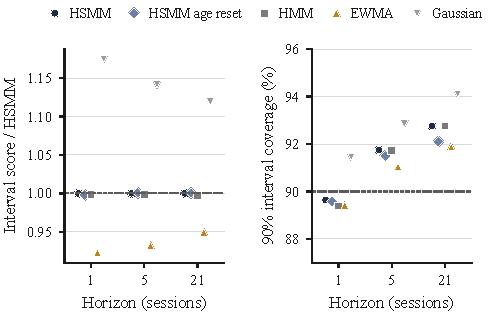
\includegraphics[width=\columnwidth]{figures/fig_scores.pdf}
\caption{Left: mean interval score of each method divided by the HSMM score at the same horizon (below 1 is better than the HSMM). Right: empirical coverage of nominal 90\% intervals; the dashed line marks 90\%.}
\label{fig:scores}
\end{figure}

EWMA had the lowest mean interval score at every horizon. The HSMM score was 8.4\%, 7.3\% and 5.3\% higher than EWMA at 1, 5 and 21 sessions. At one session the two methods produced the same mean width, 0.0347, so the EWMA advantage comes from smaller penalties for outcomes outside the interval. The HSMM and the matched HMM differed by at most 0.36\%. Both improved on the unconditional Gaussian baseline, by 10.7\% to 15.0\% depending on method and horizon. On non-overlapping 21-session origins ($n=227$), the scores were 0.19905 (HSMM), 0.19910 (age reset), 0.19934 (HMM), 0.18722 (EWMA) and 0.23273 (Gaussian), which preserves the ranking.

Brier scores for the loss probability lie between 0.2385 and 0.2500 for all methods. A constant forecast of 0.5 scores 0.25, which is exactly the EWMA value. None of the models provides a materially informative probability of a loss over these horizons.

\begin{table}[t]
\centering
\caption{Paired interval-score differences, HSMM minus baseline}
\label{tab:paired}
\footnotesize
\setlength{\tabcolsep}{5pt}
\begin{tabular}{@{}llrc@{}}
\toprule
$h$ & Baseline & $\bar\delta\times 10^{3}$ & 95\% block-bootstrap interval \\
\midrule
1 & HMM & 0.079 & $[-0.048,\ 0.196]$ \\
  & HSMM age reset & 0.109 & $[0.021,\ 0.198]$ \\
  & EWMA & 4.025 & $[0.309,\ 9.949]$ \\
  & Gaussian & $-9.089$ & $[-11.708,\ -6.255]$ \\
\midrule
5 & HMM & 0.137 & $[-0.223,\ 0.547]$ \\
  & HSMM age reset & $-0.084$ & $[-0.630,\ 0.481]$ \\
  & EWMA & 7.194 & $[2.752,\ 12.702]$ \\
  & Gaussian & $-14.973$ & $[-21.242,\ -8.334]$ \\
\midrule
21 & HMM & 0.750 & $[-0.713,\ 2.430]$ \\
  & HSMM age reset & $-0.094$ & $[-2.419,\ 2.110]$ \\
  & EWMA & 10.726 & $[-0.961,\ 21.762]$ \\
  & Gaussian & $-25.305$ & $[-38.629,\ -10.448]$ \\
\bottomrule
\end{tabular}

\vspace{2pt}
\parbox{\columnwidth}{\scriptsize Positive values mean the HSMM scored worse. Intervals use 63-session blocks and 500 resamples.}
\end{table}

\subsection{Paired comparisons}
Table~\ref{tab:paired} gives the paired differences. Against the matched HMM, every interval contains zero. Against EWMA, the HSMM is worse and the interval excludes zero at 1 and 5 sessions. At 21 sessions the mean difference is larger, $10.7\times10^{-3}$, but the interval $[-0.96, 21.76]\times10^{-3}$ includes zero, reflecting fewer effectively independent 21-session outcomes. The HSMM is better than the Gaussian baseline at every horizon. The age-reset ablation isolates the duration information. At one session, conditioning on age made the score slightly worse, by $0.109\times10^{-3}$ with an interval that excludes zero. At 5 and 21 sessions the difference is indistinguishable from zero. We found no evidence that elapsed age improved interval forecasts.

\subsection{Results by state}
Table~\ref{tab:state} conditions on the HSMM's most probable state at the origin; the same origins are used for every method. In Low and Elevated states at one session, the HSMM, HMM and EWMA scores agree to within $0.6\times10^{-3}$. The EWMA advantage is concentrated in Stress, where its one-session score is 0.08485 against 0.10233 for the HSMM. The Gaussian baseline covers only 73.86\% of one-session outcomes in Stress, while the HSMM, age-reset, HMM and EWMA methods cover between 88.86\% and 89.21\%. In Low volatility at 21 sessions, the HSMM lower breach rate is 8.51\%, the largest of any state.

\begin{table}[t]
\centering
\caption{Mean interval score by filtered HSMM state at the origin}
\label{tab:state}
\footnotesize
\setlength{\tabcolsep}{4.5pt}
\begin{tabular}{@{}llrrr@{}}
\toprule
$h$ & Method & Low vol. & Elevated & Stress \\
\midrule
1 & HSMM & 0.02973 & 0.04330 & 0.10233 \\
  & HMM & 0.02961 & 0.04323 & 0.10230 \\
  & EWMA & 0.02962 & 0.04382 & 0.08485 \\
  & Gaussian & 0.04236 & 0.04593 & 0.11499 \\
\midrule
21 & HSMM & 0.14020 & 0.20708 & 0.33970 \\
  & HMM & 0.14036 & 0.20669 & 0.33687 \\
  & EWMA & 0.12926 & 0.19664 & 0.32890 \\
  & Gaussian & 0.19325 & 0.22255 & 0.33233 \\
\bottomrule
\end{tabular}

\vspace{2pt}
\parbox{\columnwidth}{\scriptsize Origins per state for $h=1$: 1,943, 1,696 and 1,140; for $h=21$: 1,938, 1,681 and 1,140.}
\end{table}

\subsection{Two forecast origins}
Fig.~\ref{fig:fans} shows 21-session scenarios from two origins. On 12 September 2008, the 2008 vintage placed the market in Stress with probability 0.9996 and an expected age of 57.5 sessions. Its 90\% interval for the 21-session return was $[-10.15\%, 12.04\%]$, close to the EWMA interval $[-10.72\%, 12.01\%]$. The realized return to 13 October 2008 was $-19.84\%$, with a low of $-28.16\%$ along the path. On 21 February 2020, the 2020 vintage assigned Elevated volatility with probability 0.983. Its interval $[-4.70\%, 7.20\%]$ again resembled EWMA's $[-5.15\%, 5.42\%]$, and the realized return to 23 March 2020 was $-32.97\%$. Both outcomes lie far outside every method's interval. The single 2020 origin has an HSMM interval score of 5.77, about 27 times the 21-session mean. A handful of such origins therefore has a large effect on the averages in Table~\ref{tab:overall}.

\begin{figure}[t]
\centering
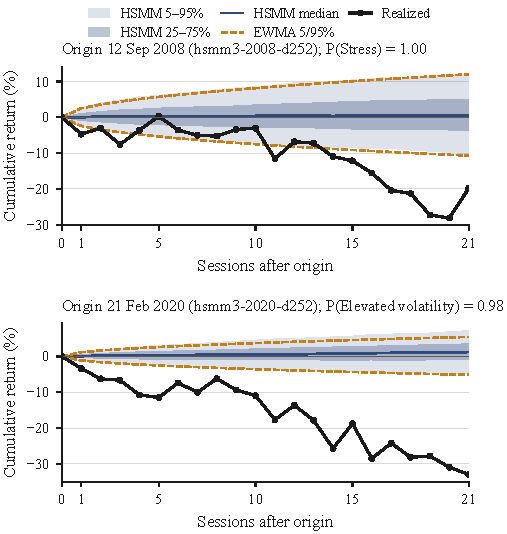
\includegraphics[width=\columnwidth]{figures/fig_fans.pdf}
\caption{HSMM 21-session scenario fans (2,000 paths) with the EWMA 90\% band and the realized cumulative return. The simulated quantiles at sessions 1, 5 and 21 equal the stored test forecasts.}
\label{fig:fans}
\end{figure}

%=====================================================================
\section{Discussion}
\label{sec:discussion}
%=====================================================================
The main result is negative. An explicit-duration model with age-aware filtering did not produce better 90\% intervals than an HMM with the same features, and both were worse than a one-parameter EWMA at short horizons. The age-reset ablation shows that the duration component itself contributed nothing measurable. We report this result because the model was designed to test exactly this mechanism.

The results suggest, but do not establish, three explanations. First, the scenario variance is tied to one of three discrete levels. Within Stress, the HSMM uses the same daily standard deviation whether VIX is 30 or 80, whereas EWMA scales immediately with the latest squared return. Table~\ref{tab:state} is consistent with this: the gap is largest in Stress. Second, at horizons of 1 to 21 sessions the forecast distribution is dominated by the current state's variance. Age changes the probability of a state change within the horizon, and its effect on the 5th and 95th percentiles of a 2,000-path mixture is small. Third, both regime models produce more lower breaches than nominal. Gaussian state-conditional returns understate the left tail. Both losses in Fig.~\ref{fig:fans} fell below every method's interval, including the one issued from Stress.

The estimated durations are nonetheless informative descriptively. The Stress dispersion of 0.48 in the 2026 vintage implies a decreasing exit hazard, which a geometric duration cannot represent. That finding concerns model fit; it did not improve forecast scores in this evaluation. The application therefore presents the HSMM as a regime-research model and displays the EWMA reference interval and the measured scores next to each scenario.

%=====================================================================
\section{Limitations}
\label{sec:limitations}
%=====================================================================
Gaussian emissions and state-marginal return draws understate tail risk, as the lower breach rates show. Only one index is studied, and the conclusions may not transfer to other assets or to portfolios. The number of states, the ten-year window and the feature set were fixed rather than validated, and only two duration caps were compared. Overlapping horizons create dependent errors. The block length of 63 sessions and the 500 bootstrap resamples were also fixed and not tuned, and the 21-session intervals are correspondingly wide. The 2013 refit was made after results were inspected. Later vintages train on earlier test years once those years have passed, which is legitimate for forecasting but means test years are not independent of later models. Prices are revised vendor data rather than a point-in-time archive. The frozen file contains five sessions with a zero log return, including 3 January 2008, that are consistent with repeated vendor closes; they were not altered. Returns exclude dividends. State probabilities are model probabilities and not classification accuracy.

%=====================================================================
\section{System Implementation}
\label{sec:system}
%=====================================================================
The application has three tiers (Fig.~\ref{fig:arch}). A React and Vite single-page client calls one Express API. Express provides the browser-facing endpoints, caches responses in memory, serves Yahoo Finance quotes and a cross-asset Macro Pulse summary, and forwards model requests to a FastAPI service. The Python service owns filtering, simulation and evaluation records; training runs offline with \texttt{python -m research.train}, and \texttt{python -m research.audit} regenerates the audit. The model code uses NumPy, SciPy, scikit-learn, hmmlearn and Numba. There is no database: model vintages, forecasts and evaluation summaries are versioned files, and the user's watchlist and positions remain in browser storage.

A snapshot is identified by a hash of the model identifier, data version, observation date, horizon and number of paths. It returns the state probabilities, expected age, next-session switch probability, scenario fan, loss probabilities, 95\% VaR and expected shortfall, together with the EWMA reference interval and the measured test scores for that horizon. An exposure calculator scales the return distribution to a dollar amount between \$1,000 and \$100,000. Historical replay loads the vintage trained strictly before the chosen date and hides the realized outcome until the user requests it. The evaluation view presents the scores, coverage, breach rates, Brier scores, state-level results and bootstrap intervals reported in Section~\ref{sec:results}.

Text explanations use a single model through OpenRouter when an API key is configured. Without a key, or when the provider fails, a rule-based analyst assembles answers from Yahoo Finance data and the current HSMM snapshot, and labels them as such. This design keeps every displayed number traceable to data or to the model. The repository's unit tests cover exact inference on small sequences, recovery of synthetic states, stability of filtered probabilities when observations are appended, artifact serialization, risk metrics and replay chronology.

%=====================================================================
\section{Conclusion}
\label{sec:conclusion}
%=====================================================================
We built and evaluated a three-state explicit-duration Gaussian HSMM for S\&P~500 volatility regimes. The model filters over state and elapsed age, handles unknown initial age and a right-censored final segment, and simulates age-conditioned scenarios. In a walk-forward test over 2007--2025, its 90\% intervals reached 89.64\% to 92.75\% coverage but did not improve on a matched HMM, and they were worse than an EWMA baseline at 1 and 5 sessions. Removing age information did not degrade the scores. The fitted durations show a decreasing exit hazard for Stress, but this property did not translate into better intervals. Future work should test heavier-tailed emissions, state-dependent variance scaling with realized volatility, and evaluation on additional indices.

%=====================================================================
\IEEEtriggeratref{16}
\begin{thebibliography}{99}
\footnotesize

\bibitem{engle1982}
R.~F. Engle, ``Autoregressive conditional heteroscedasticity with estimates of the variance of United Kingdom inflation,'' \emph{Econometrica}, vol.~50, no.~4, pp.~987--1007, 1982.

\bibitem{bollerslev1986}
T.~Bollerslev, ``Generalized autoregressive conditional heteroskedasticity,'' \emph{J. Econometrics}, vol.~31, no.~3, pp.~307--327, 1986.

\bibitem{hamilton1989}
J.~D. Hamilton, ``A new approach to the economic analysis of nonstationary time series and the business cycle,'' \emph{Econometrica}, vol.~57, no.~2, pp.~357--384, 1989.

\bibitem{ang2012}
A.~Ang and A.~Timmermann, ``Regime changes and financial markets,'' \emph{Annu. Rev. Financial Econ.}, vol.~4, pp.~313--337, 2012.

\bibitem{ryden1998}
T.~Ryd\'en, T.~Ter\"asvirta, and S.~\AA{}sbrink, ``Stylized facts of daily return series and the hidden Markov model,'' \emph{J. Appl. Econometrics}, vol.~13, no.~3, pp.~217--244, 1998.

\bibitem{bulla2006}
J.~Bulla and I.~Bulla, ``Stylized facts of financial time series and hidden semi-Markov models,'' \emph{Comput. Statist. Data Anal.}, vol.~51, no.~4, pp.~2192--2209, 2006.

\bibitem{rabiner1989}
L.~R. Rabiner, ``A tutorial on hidden Markov models and selected applications in speech recognition,'' \emph{Proc. IEEE}, vol.~77, no.~2, pp.~257--286, 1989.

\bibitem{dempster1977}
A.~P. Dempster, N.~M. Laird, and D.~B. Rubin, ``Maximum likelihood from incomplete data via the EM algorithm,'' \emph{J. Roy. Statist. Soc. B}, vol.~39, no.~1, pp.~1--38, 1977.

\bibitem{yu2010}
S.-Z. Yu, ``Hidden semi-Markov models,'' \emph{Artif. Intell.}, vol.~174, no.~2, pp.~215--243, 2010.

\bibitem{guedon2003}
Y.~Gu\'edon, ``Estimating hidden semi-Markov chains from discrete sequences,'' \emph{J. Comput. Graph. Statist.}, vol.~12, no.~3, pp.~604--639, 2003.

\bibitem{riskmetrics1996}
J.~P. Morgan and Reuters, \emph{RiskMetrics---Technical Document}, 4th~ed. New York, NY, USA: J.~P. Morgan, 1996.

\bibitem{gneiting2007}
T.~Gneiting and A.~E. Raftery, ``Strictly proper scoring rules, prediction, and estimation,'' \emph{J. Amer. Statist. Assoc.}, vol.~102, no.~477, pp.~359--378, 2007.

\bibitem{christoffersen1998}
P.~F. Christoffersen, ``Evaluating interval forecasts,'' \emph{Int. Econ. Rev.}, vol.~39, no.~4, pp.~841--862, 1998.

\bibitem{brier1950}
G.~W. Brier, ``Verification of forecasts expressed in terms of probability,'' \emph{Monthly Weather Rev.}, vol.~78, no.~1, pp.~1--3, 1950.

\bibitem{diebold1995}
F.~X. Diebold and R.~S. Mariano, ``Comparing predictive accuracy,'' \emph{J. Bus. Econ. Statist.}, vol.~13, no.~3, pp.~253--263, 1995.

\bibitem{kunsch1989}
H.~R. K\"unsch, ``The jackknife and the bootstrap for general stationary observations,'' \emph{Ann. Statist.}, vol.~17, no.~3, pp.~1217--1241, 1989.

\bibitem{politis1994}
D.~N. Politis and J.~P. Romano, ``The stationary bootstrap,'' \emph{J. Amer. Statist. Assoc.}, vol.~89, no.~428, pp.~1303--1313, 1994.

\bibitem{artzner1999}
P.~Artzner, F.~Delbaen, J.-M. Eber, and D.~Heath, ``Coherent measures of risk,'' \emph{Math. Finance}, vol.~9, no.~3, pp.~203--228, 1999.

\bibitem{cboevix}
Cboe Global Markets, ``VIX index historical data.'' [Online]. Available: \url{https://www.cboe.com/tradable-products/vix/vix-historical-data}. Accessed: Nov.~2, 2026.

\bibitem{fred}
Federal Reserve Bank of St.~Louis, ``S\&P 500 (SP500),'' FRED. [Online]. Available: \url{https://fred.stlouisfed.org/series/SP500}. Accessed: Nov.~2, 2026.

\end{thebibliography}

\end{document}
